\documentclass{article}
\usepackage{CJKutf8}
\usepackage{graphicx}
\usepackage{amsthm}
\let\proof\relax \let\endproof\relax % 避免 math_blog 重复定义 proof 报错
\usepackage{math_blog}
\usepackage{amsmath}
\usepackage{appendix}
\usepackage[normalem]{ulem}
\usepackage[thicklines]{cancel}
\usepackage{tikz}
\usetikzlibrary{positioning,arrows.meta}
\usepackage{pgfplots}

% Defensive: resolve possible \proof / theorem-env conflicts with math_blog
\makeatletter
\@ifundefined{proof}{}{\let\proof\@undefined \let\endproof\@undefined}
\@ifundefined{theorem}{\newtheorem{theorem}{Theorem}[section]}{}
\@ifundefined{lemma}{\newtheorem{lemma}[theorem]{Lemma}}{}
\@ifundefined{definition}{\newtheorem{definition}[theorem]{Definition}}{}
\makeatother
\newenvironment{proof}[1][证明]{%
  \par\smallskip\noindent\textit{\textbf{#1.}}\quad\ignorespaces
}{%
  \hfill$\square$\par\smallskip
}

% 中文环境名（与 theorem 共用计数器）
\theoremstyle{plain}
\newtheorem{zhtheorem}[theorem]{定理}
\newtheorem{zhlemma}[theorem]{引理}
\theoremstyle{definition}
\newtheorem{zhdefinition}[theorem]{定义}
\let\theorem\zhtheorem \let\endtheorem\endzhtheorem
\let\lemma\zhlemma \let\endlemma\endzhlemma
\let\definition\zhdefinition \let\enddefinition\endzhdefinition
\renewcommand{\figurename}{图}
\renewcommand{\tablename}{表}

\title{[SDE III] 存在唯一性与 SDE--PDE 之间的桥梁}
\author{Anqiao Ouyang, Xuecheng Liu}
\date{May 26, 2026}

\newcommand{\Title}{存在唯一性与 SDE--PDE 之间的桥梁}

\newcommand{\Column}{Stochastic Differential Equations III}
\newcommand{\Author}{Anqiao Ouyang}

\begin{document}
\begin{CJK*}{UTF8}{gbsn}

\maketitle

\section{引言}

在前两篇文章里，我们把布朗运动当作连续但处处不可微的驱动过程，把 It\^o 积分作为对它做积分的正确方式，再用 It\^o 公式作为随机动力学的链式法则。我们还讨论了若干数值格式（Euler--Maruyama、Milstein），过程中用到了一些\textbf{只陈述未严格证明}的结果，例如解的存在性、马尔可夫性，以及作用在条件期望上的抛物算子 $\partial_t+\mathcal L$。

本文把这些坑补上，并往前再走一步。我们要回答三个相互交织的问题：
\begin{enumerate}
    \item SDE
    \[
      \mathrm{d}X_t=a(t,X_t)\,\mathrm{d}t+b(t,X_t)\,\mathrm{d}B_t,\qquad X_0=x_0
    \]
    在什么条件下有解？解唯一吗？这里说的“解”究竟是什么意思？
    \item 解一旦存在，它的概率结构是怎样的？尤其，为什么它是马尔可夫的？应该用哪个对象来读取 $X_t$ 的分布？
    \item SDE 是怎么跟确定性 PDE 联系的？条件期望 $u(t,x)=\mathbb{E}[f(X_T)\mid X_t=x]$ 在 II 篇里已经出现在 EM 格式的弱收敛证明里；这里要解释为什么它满足一个抛物方程，推出边际密度的 Fokker--Planck 方程，并把一切跟 Feynman--Kac 公式以及 Girsanov 定理串起来。
\end{enumerate}

把这些主题串成一线的，是\textbf{无穷小生成元}
\[
  \mathcal L=a\,\partial_x+\tfrac12 b^2\,\partial^2_{xx}.
\]
它编码了 SDE；它决定转移半群；它是 Kolmogorov 两个方程里的空间算子；而 Feynman--Kac 本质上是在说 $\partial_t+\mathcal L$ 有一个随机表示。

\section{存在性与唯一性}

\subsection{强解与弱解}

SDE 理论里同时存在两种“解”的概念，它们回答的是不同的问题。

\begin{definition}[强解]
固定概率空间 $(\Omega,\mathcal{F},\mathbb{P})$、布朗运动 $B$，以及由 $B$ 生成（并完备化以满足通常条件）的流 $\{\mathcal{F}_t\}$。SDE
\begin{equation}\label{eq:sde}
    \mathrm{d}X_t=a(t,X_t)\,\mathrm{d}t+b(t,X_t)\,\mathrm{d}B_t,\qquad X_0=\xi,
\end{equation}
的\textbf{强解}是一个 $\{\mathcal{F}_t\}$-适应、几乎处处连续的过程 $X$，满足
\[
  X_t=\xi+\int_0^t a(s,X_s)\,\mathrm{d}s+\int_0^t b(s,X_s)\,\mathrm{d}B_s,\qquad \forall t\in[0,T]\ \text{a.s.}
\]
\end{definition}

通俗地说：驱动 $B$ 是先给定的，解是它路径的一个可测泛函。需要做模拟时这个观点最合适，因为 EM 格式正是逐路径地从单条布朗轨道构造 $\bar{X}^\delta$。

\begin{definition}[弱解]
一组\textbf{弱解}指的是一个元组 $(\Omega,\mathcal{F},\mathbb{P},\{\mathcal{F}_t\},B,X)$，其中 $B$ 是这个空间上的 $\{\mathcal{F}_t\}$-布朗运动，且 $X$ 满足上述积分方程。这里布朗运动和概率空间都是“答案”的一部分，而非问题的前提。
\end{definition}

要研究 $X$ 的\emph{分布}（分布性质、矩、转移概率），弱解就够了，因为我们可以挑一个方便的空间。但要研究 $X$ 跟某条特定 $B$ 之间的关系（模拟、滤波、逐路径控制），就必须用强解。

强解必然也是弱解，反之未必。存在只有弱解、没有强解的 SDE：经典反例是 Tanaka 方程 $\mathrm{d}X_t=\operatorname{sgn}(X_t)\,\mathrm{d}B_t$。本文以下专注于强解，因为标准的 Lipschitz 框架可以直接给出它。

\subsection{Picard--Lindel\"of 论证的随机版本}

确定性情形下，对 $\dot x=f(t,x)$（关于 $x$ 是 Lipschitz）证明存在唯一性用 Picard 迭代：定义 $x^{(n+1)}_t=x_0+\int_0^t f(s,x^{(n)}_s)\,\mathrm{d}s$，证明 $\{x^{(n)}\}$ 在 $C([0,T])$ 中是 Cauchy 列。随机版本骨架相同，只是用 $L^2(\Omega)$ 估计代替逐点估计，关键的扩散项靠 It\^o 等距撑场面。

把假设统一列出来。下面这些就是 II 篇里讨论 EM 收敛时\emph{暗中}用到的 Condition 1--4：

\begin{itemize}
    \item \textbf{(L) Lipschitz：}存在 $L>0$ 使得
    $|a(t,x)-a(t,y)|+|b(t,x)-b(t,y)|\le L|x-y|$，对所有 $t\in[0,T]$，$x,y\in\mathbb{R}$ 成立。
    \item \textbf{(G) 线性增长：}存在 $C>0$ 使得
    $|a(t,x)|^2+|b(t,x)|^2\le C(1+|x|^2)$。
    \item \textbf{(I) 初值：}$\xi$ 是 $\mathcal{F}_0$-可测的，且 $\mathbb{E}|\xi|^2<\infty$。
\end{itemize}

\begin{theorem}[强解的存在与唯一]\label{thm:exuniq}
在 (L)、(G)、(I) 下，SDE \eqref{eq:sde} 存在唯一一个强解 $X\in L^2_T(\Omega)$，路径连续。而且
\[
  \mathbb{E}\!\left[\sup_{0\le t\le T}|X_t|^2\right]\le K\,(1+\mathbb{E}|\xi|^2),
\]
其中常数 $K$ 只依赖 $L,C,T$。
\end{theorem}

证明分三步：先验矩估计、Picard 序列的 Cauchy 性、逐路径唯一性。这里只勾出骨架，细节见附录~\ref{app:exuniq}。

\paragraph{Step 1：先验估计。} 定义算子 $\Phi:L^2_T(\Omega)\to L^2_T(\Omega)$：
\[
  (\Phi X)_t=\xi+\int_0^t a(s,X_s)\,\mathrm{d}s+\int_0^t b(s,X_s)\,\mathrm{d}B_s.
\]
要证 $\Phi$ 把 $L^2_T$ 映到自身。漂移项用 Cauchy--Schwarz，扩散项用 It\^o 等距：
\[
  \mathbb{E}|(\Phi X)_t|^2\le 3\mathbb{E}|\xi|^2+3T\,\mathbb{E}\!\int_0^t|a(s,X_s)|^2\,\mathrm{d}s+3\,\mathbb{E}\!\int_0^t|b(s,X_s)|^2\,\mathrm{d}s.
\]
代入 (G)：
\[
  \mathbb{E}|(\Phi X)_t|^2\le 3\mathbb{E}|\xi|^2+3(T+1)C\!\int_0^t\!\bigl(1+\mathbb{E}|X_s|^2\bigr)\,\mathrm{d}s,
\]
对 $X\in L^2_T$ 是有限的。要从逐点矩估计升级为定理里那个一致 $\sup$ 界，对扩散积分用 Doob 的 $L^2$ 极大不等式，再对 $\psi(t)=\mathbb{E}\sup_{s\le t}|X_s|^2$ 用 Gronwall。

\paragraph{Step 2：Picard 迭代。} 令 $X^{(0)}_t\equiv\xi$，$X^{(n+1)}=\Phi X^{(n)}$。利用 Lipschitz 条件 (L) 做标准计算：
\[
  \mathbb{E}\!\left[\sup_{s\le t}|X^{(n+1)}_s-X^{(n)}_s|^2\right]\le K_1\!\int_0^t\mathbb{E}\!\left[\sup_{r\le s}|X^{(n)}_r-X^{(n-1)}_r|^2\right]\mathrm{d}s.
\]
Doob 的 $L^2$ 极大不等式让我们能把 $\sup$ 移到扩散项的期望里面。迭代 $n$ 次：
\[
  \mathbb{E}\!\left[\sup_{s\le T}|X^{(n+1)}_s-X^{(n)}_s|^2\right]\le \frac{(K_1 T)^n}{n!}\,M_0,
\]
其中 $M_0=\mathbb{E}\sup_{s\le T}|X^{(1)}_s-X^{(0)}_s|^2<\infty$。级数 $\sum_n \sqrt{(K_1T)^n/n!}$ 收敛，故 $\{X^{(n)}\}$ 在 Banach 空间 $\mathcal{S}^2_T$（适应、连续过程，范数 $\|X\|_{\mathcal{S}^2}=\bigl(\mathbb{E}\sup_{s\le T}|X_s|^2\bigr)^{1/2}$）中是 Cauchy 列，极限 $X$ 就是强解。

\paragraph{Step 3：唯一性。} 设 $X,Y$ 都是 \eqref{eq:sde} 的解。对差 $X-Y$ 重做 Step 2 的估计，再调用 Gronwall（附录~\ref{app:gronwall}）得到 $\mathbb{E}\sup_{s\le T}|X_s-Y_s|^2=0$，故 $X=Y$ 不可区分。

\medskip

几点补充：

\begin{itemize}
    \item \textbf{Lipschitz 条件可大幅弱化。}\textbf{Yamada--Watanabe} 定理给出 1D SDE 的逐路径唯一性，只要 $|b(x)-b(y)|\le h(|x-y|)$ 对某个递增函数 $h:(0,\infty)\to(0,\infty)$ 成立，且 $\int_{0+}h^{-2}(u)\,\mathrm{d}u=\infty$；这覆盖了 H\"older 指数 $\alpha\ge 1/2$ 的情形。CIR 模型里的开方项 $\mathrm{d}X_t=\kappa(\theta-X_t)\,\mathrm{d}t+\sigma\sqrt{X_t}\,\mathrm{d}B_t$ 恰好踩在 H\"older $1/2$ 这条边界上。它\emph{不是} Lipschitz 的，但 Yamada--Watanabe 仍然给出唯一性。
    \item \textbf{没有线性增长，解可能在有限时间内爆掉。}\textbf{爆炸时间}
    $\tau_\infty=\lim_{n\to\infty}\inf\{t:|X_t|\ge n\}$
    可能几乎处处有限。即使是无噪声的 ODE $\dot X_t=X_t^2$（$X_0>0$）也会在 $t=1/X_0$ 爆掉。标准做法是局部化：先解到 $\tau_n$，再验证 $\mathbb{P}(\tau_\infty>T)=1$。
    \item \textbf{(G) 本质上是矩控制的紧界。}没有它，即使逐路径有解，$\mathbb{E}|X_t|^2$ 也可能发散。
\end{itemize}

\section{马尔可夫性与生成元}

\subsection{马尔可夫性}

确定性 ODE $\dot x=f(t,x)$ 有平凡的流性质：$s$ 时刻以后的轨道只依赖 $x_s$，跟更早的历史无关。时齐 SDE 的解也是如此，只是“只依赖 $X_s$”这句话必须从“函数值相等”升级为“条件\emph{分布}相等”。

\begin{theorem}[马尔可夫性]\label{thm:markov}
设 $X$ 是 \eqref{eq:sde} 的强解，系数 $a(x),b(x)$ 时齐且 Lipschitz。则对任意有界可测函数 $f:\mathbb{R}\to\mathbb{R}$ 与 $0\le s\le t\le T$，
\[
  \mathbb{E}\bigl[f(X_t)\mid \mathcal{F}_s\bigr]=\mathbb{E}\bigl[f(X_t)\mid X_s\bigr]\qquad\text{a.s.}
\]
\end{theorem}

\begin{proof}[证明（梗概）]
关键观察是：从时间 $s$ 起、初值为 $X_s$ 的 SDE 解，只依赖布朗增量 $B_u-B_s$（$u\ge s$），而这些增量与 $\mathcal{F}_s$ 独立。把 $X_t=\Psi(s,t,X_s,(B_u-B_s)_{s\le u\le t})$ 写出来（$\Psi$ 是把初值和驱动路径映到解的\emph{确定性}泛函，由存在唯一性以及 Picard 迭代的逐路径性质保证良定），就有 $\mathbb{E}[f(X_t)\mid\mathcal{F}_s]=\Phi(X_s)$，其中
\[
  \Phi(x)=\mathbb{E}\bigl[f(\Psi(s,t,x,(B_u-B_s)_{s\le u\le t}))\bigr].
\]
右侧是 $x$ 的确定性函数，于是 $\sigma(X_s)$-可测，根据塔性质就等于 $\mathbb{E}[f(X_t)\mid X_s]$。
\end{proof}

时非齐 SDE 的解依然是马尔可夫的，只不过转移概率依赖两个端点 $(s,t)$，而非时间差 $t-s$。

\subsection{转移算子半群}

马尔可夫性鼓励一种泛函分析的重新表述。在时齐情形下，定义算子 $P_t:B_b(\mathbb{R})\to B_b(\mathbb{R})$（有界可测函数空间）：
\[
  P_t f(x)=\mathbb{E}_x[f(X_t)]:=\mathbb{E}\bigl[f(X_t)\mid X_0=x\bigr].
\]
根据马尔可夫性和时齐性，$\{P_t\}_{t\ge 0}$ 是一个\textbf{半群}：
\[
  P_{t+s}f(x)=\mathbb{E}_x[f(X_{t+s})]=\mathbb{E}_x[\mathbb{E}[f(X_{t+s})\mid\mathcal{F}_s]]=\mathbb{E}_x[P_t f(X_s)]=P_s(P_t f)(x).
\]
$P_t f$ 是一个新的可观测量，它在 $x$ 处的值是从 $x$ 出发、经过 $t$ 时间之后 $f$ 的期望值。半群是\emph{向前}的；“向后” Kolmogorov 方程之所以叫“向后”，是因为它从终值数据向更早时刻求解，跟 $\{P_t\}$ 的方向无关。

\subsection{无穷小生成元}

研究半群的自然工具是它的无穷小生成元。启发性地，
\[
  \mathcal{L}f(x)=\lim_{t\downarrow 0}\frac{P_t f(x)-f(x)}{t}.
\]
对系数光滑的 SDE，生成元就是我们一直在写的那个抛物算子。

\begin{theorem}[It\^o 扩散的生成元]\label{thm:generator}
设 $X$ 解 $\mathrm{d}X_t=a(X_t)\,\mathrm{d}t+b(X_t)\,\mathrm{d}B_t$，$a,b$ Lipschitz，$f\in C^2_b(\mathbb{R})$。则
\[
  \mathcal{L}f(x)=a(x)f'(x)+\tfrac{1}{2}b^2(x)f''(x),
\]
且极限关于 $x$ 一致成立。
\end{theorem}

\begin{proof}
对 $f(X_t)$ 用 It\^o 公式（$X_0=x$）：
\[
  f(X_t)-f(x)=\int_0^t \bigl(a f'+\tfrac{1}{2}b^2 f''\bigr)(X_s)\,\mathrm{d}s+\int_0^t b(X_s)f'(X_s)\,\mathrm{d}B_s.
\]
取期望，随机积分项消失（其被积函数属于 $L^2_T$：$f',b$ 在 $X_s$（$s\in[0,t]$）的值域上有界，由线性增长保证可积性）。除以 $t$：
\[
  \frac{P_tf(x)-f(x)}{t}=\frac{1}{t}\mathbb{E}_x\!\int_0^t\mathcal{L}f(X_s)\,\mathrm{d}s\xrightarrow{t\downarrow 0}\mathcal{L}f(x),
\]
这是因为 $\mathcal{L}f(X_s)$ 关于 $s$ 连续（$X$ 连续，$\mathcal{L}f$ 连续有界）。
\end{proof}

\begin{figure}[htbp]
\centering
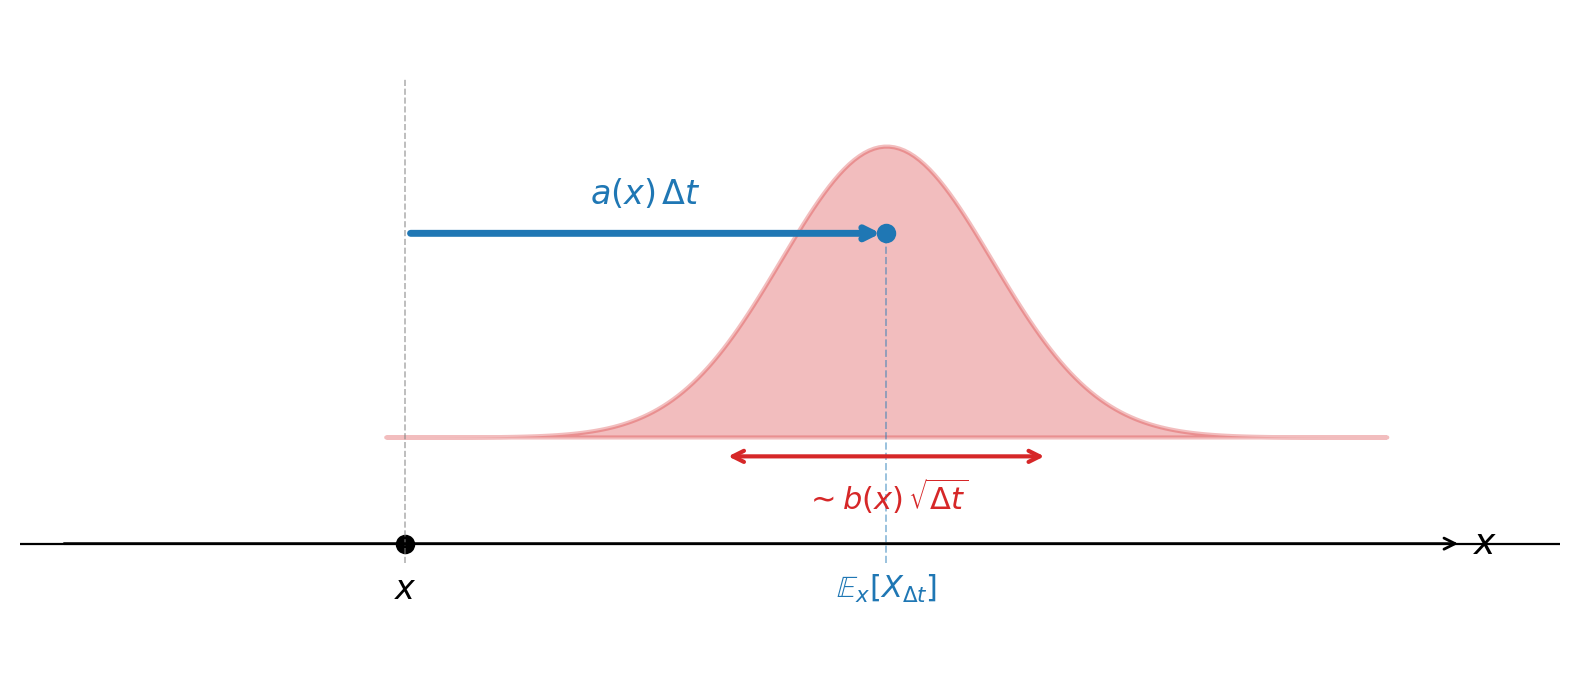
\includegraphics[width=0.85\linewidth]{figures/fig1_generator.png}
\caption{生成元 $\mathcal{L}=a\partial_x+\tfrac{1}{2}b^2\partial_{xx}^2$ 的局部图像。从 $x$ 出发，经过一小段时间 $\Delta t$，蓝色箭头是 $a(x)\Delta t$ 量级的漂移（确定性位移）；红色 Gaussian 云是 $b(x)\sqrt{\Delta t}$ 量级的扩散波动。$\Delta t$ 很小时 $\sqrt{\Delta t}\gg\Delta t$，扩散占主导，因此 $\mathcal L$ 必须含有二阶项，其系数 $\tfrac12 b^2$ 正好与方差的 $\Delta t$ 标度相匹配。}
\label{fig:generator}
\end{figure}

注意这个不对称：漂移贡献一阶项，扩散贡献二阶项。这直接来自 It\^o 计算的恒等式 $(\mathrm{d}B_t)^2=\mathrm{d}t$——扩散在无穷小尺度上“跑得比漂移快两倍”，这就是 $\tfrac{1}{2}b^2$ 系数的来源。

\section{Kolmogorov 向后与向前方程}

生成元 $\mathcal{L}$ 主宰两个互为对偶的 PDE，它们完整刻画了 $X$ 的分布。

\subsection{向后方程}

固定终止时间 $T$ 和支付函数 $f\in C_b(\mathbb{R})$。定义
\[
  u(t,x)=\mathbb{E}\bigl[f(X_T)\mid X_t=x\bigr]=P_{T-t}f(x).
\]
这个条件期望在 II 篇 EM 弱收敛证明里已经出现过。向后方程说，它满足一个确定性 PDE。

\begin{theorem}[Kolmogorov 向后方程]\label{thm:backward}
设 $a,b$ Lipschitz 且各阶导数有界，$f\in C^2_P$（多项式增长）。则 $u(t,x)=\mathbb{E}_{t,x}[f(X_T)]$ 属于 $C^{1,2}([0,T)\times\mathbb{R})$，且满足
\[
  \begin{cases}
    \partial_t u(t,x)+\mathcal{L}u(t,x)=0,& (t,x)\in[0,T)\times\mathbb{R},\\
    u(T,x)=f(x).
  \end{cases}
\]
\end{theorem}

\begin{proof}[证明（梗概）]
对 $u(s,X_s)$ 在 $s\in[t,T]$ 上用 It\^o 公式，条件在 $X_t=x$ 下：
\[
  u(T,X_T)-u(t,x)=\int_t^T(\partial_s u+\mathcal{L}u)(s,X_s)\,\mathrm{d}s+\int_t^T b(X_s)\partial_x u(s,X_s)\,\mathrm{d}B_s.
\]
取条件期望 $\mathbb{E}_{t,x}$：扩散项均值为零（由 $\partial_x u$ 的多项式增长配上矩估计保证）。左边 $\mathbb{E}_{t,x}[f(X_T)]-u(t,x)=0$（按 $u$ 的定义）。所以
\[
  \mathbb{E}_{t,x}\!\int_t^T(\partial_s u+\mathcal{L}u)(s,X_s)\,\mathrm{d}s=0
\]
对所有 $(t,x)$ 成立。在 $s=t$ 处对 $t$ 求导并利用连续性，就得到 $(\partial_t u+\mathcal{L}u)(t,x)=0$。边值 $u(T,x)=f(x)$ 显然。

正则性 $u\in C^{1,2}$ 是难的那一步，所以我们假设了 $a,b$ 各阶导数有界。可以靠 SDE 对 $x$ 求导（\textbf{随机流}方法）来证，或者直接调用一致抛物 PDE 的标准理论。
\end{proof}

之所以叫“向后”，是因为这个 PDE 在从终值 $T$ 向后流动的时间变量里演化：当 $t$ 从 $T$ 减小，我们对 $f(X_T)$ 的信息越来越多。

\subsection{向前方程（Fokker--Planck）}

如果反过来固定初值分布 $X_0\sim\rho_0$，问 $X_t$ 的密度 $\rho(t,x)$ 满足什么方程，就得到对偶的那条 PDE。

\begin{theorem}[Fokker--Planck 方程]\label{thm:fpe}
设 $X_t$ 对每个 $t>0$ 有光滑密度 $\rho(t,x)$（例如 $b^2$ 一致椭圆，即 $b^2\ge\beta>0$ 时成立）。则 $\rho$ 满足
\[
  \partial_t\rho(t,x)=-\partial_x\bigl(a(x)\rho(t,x)\bigr)+\tfrac{1}{2}\,\partial_{xx}^2\bigl(b^2(x)\rho(t,x)\bigr)=\mathcal{L}^*\rho,
\]
初值 $\rho(0,\cdot)=\rho_0$。
\end{theorem}

\begin{proof}[证明（梗概）]
取任意测试函数 $\varphi\in C_c^\infty(\mathbb{R})$。由 It\^o 公式，
\[
  \mathbb{E}\varphi(X_t)-\mathbb{E}\varphi(X_0)=\mathbb{E}\!\int_0^t\mathcal{L}\varphi(X_s)\,\mathrm{d}s.
\]
对 $t$ 求导：
\[
  \frac{\mathrm{d}}{\mathrm{d}t}\!\int\varphi(x)\rho(t,x)\,\mathrm{d}x=\int\mathcal{L}\varphi(x)\rho(t,x)\,\mathrm{d}x=\int\varphi(x)\,\mathcal{L}^*\rho(t,x)\,\mathrm{d}x,
\]
其中分部积分两次定义了形式伴随 $\mathcal{L}^*\rho=-\partial_x(a\rho)+\tfrac{1}{2}\partial_{xx}^2(b^2\rho)$。$\varphi$ 任意，所以 $\partial_t\rho=\mathcal{L}^*\rho$（分布意义下）；$\rho$ 光滑时就升级为经典 PDE。
\end{proof}

\begin{figure}[htbp]
\centering
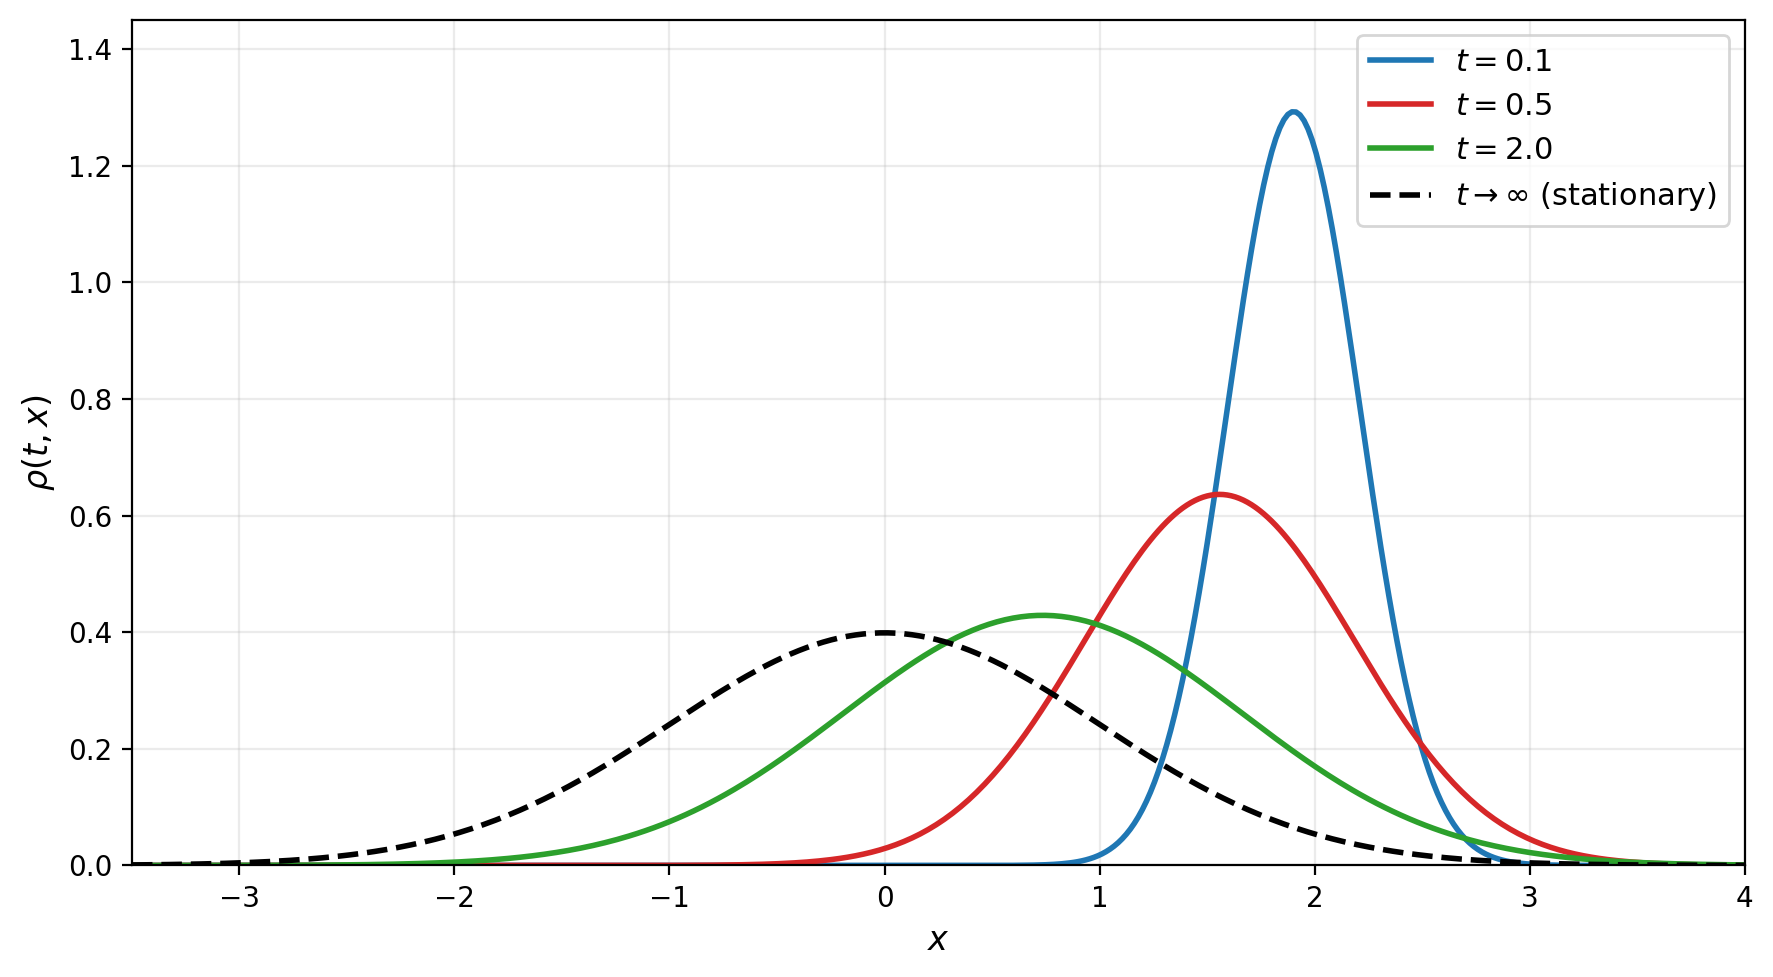
\includegraphics[width=0.85\linewidth]{figures/fig2_fokker_planck.png}
\caption{OU 过程 $\mathrm{d}X_t=-\tfrac{1}{2}X_t\,\mathrm{d}t+\mathrm{d}B_t$（$X_0=2$，Dirac 质量）的 Fokker--Planck 解。密度以速率 $\theta$ 向均值 $\mu=0$ 平移、以速率 $\sigma$ 展开，最终松弛到平稳分布 $\mathcal{N}(0,1)$（虚线）。两种运动都编码在 $\mathcal{L}^*$ 中：$-\partial_x(a\rho)$ 项搬运质量，$\tfrac12\partial^2_{xx}(b^2\rho)$ 项把它摊开。}
\label{fig:fpe}
\end{figure}

\subsection{向后 vs 向前对比一览}

把两个方程并排放在一起看：
\begin{center}
\begin{tabular}{l|ll}
  & 向后（Kolmogorov） & 向前（Fokker--Planck）\\
  \hline
  未知量 & $u(t,x)=\mathbb{E}_{t,x}[f(X_T)]$ & $\rho(t,x)$：$X_t$ 的密度\\
  PDE & $\partial_t u+\mathcal{L}u=0$ & $\partial_t\rho=\mathcal{L}^*\rho$\\
  数据 & 终值 $u(T,\cdot)=f$ & 初值 $\rho(0,\cdot)=\rho_0$\\
  $\mathcal{L}$ 中的变量 & 起点 $x$ & 当前点 $x$\\
  时间方向 & 从 $T$ 向后 & 从 $0$ 向前
\end{tabular}
\end{center}

这个二分法正是 Schr\"odinger 与 Heisenberg 表象、协变与逆变演化之间的标准二分：$u$ 演化的是可观测量，$\rho$ 演化的是状态，两个算子 $\mathcal{L},\mathcal{L}^*$ 在配对 $\langle u,\rho\rangle=\int u\rho\,\mathrm{d}x$ 下互为对偶。

\subsection{平稳分布}

\textbf{平稳}（或\textbf{不变}）分布 $\pi$ 满足 $\mathcal{L}^*\pi=0$。若 $X_0\sim\pi$，则 $X_t\sim\pi$ 对所有 $t$ 成立。

1D SDE 的平稳密度（存在且可积时）有显式公式。从 $\mathcal{L}^*\pi=-\partial_x(a\pi)+\tfrac12\partial_{xx}^2(b^2\pi)=0$ 积分一次得一阶 ODE：
\[
  \tfrac{1}{2}\,(b^2\pi)'-a\pi=\text{常数}.
\]
对于在无穷远处衰减的平稳密度，常数为零。这给出
\[
  \pi(x)\propto\frac{1}{b^2(x)}\exp\!\left(\int^x \frac{2a(y)}{b^2(y)}\,\mathrm{d}y\right).
\]

\paragraph{例：OU 过程。} 对 $\mathrm{d}X_t=\theta(\mu-X_t)\,\mathrm{d}t+\sigma\,\mathrm{d}B_t$，公式给出
\[
  \pi(x)\propto\exp\!\left(-\frac{\theta(x-\mu)^2}{\sigma^2}\right),
\]
即 $\mathcal{N}(\mu,\sigma^2/(2\theta))$，恰好对应 II 篇用显式解推出的长时间极限。

\begin{figure}[htbp]
\centering
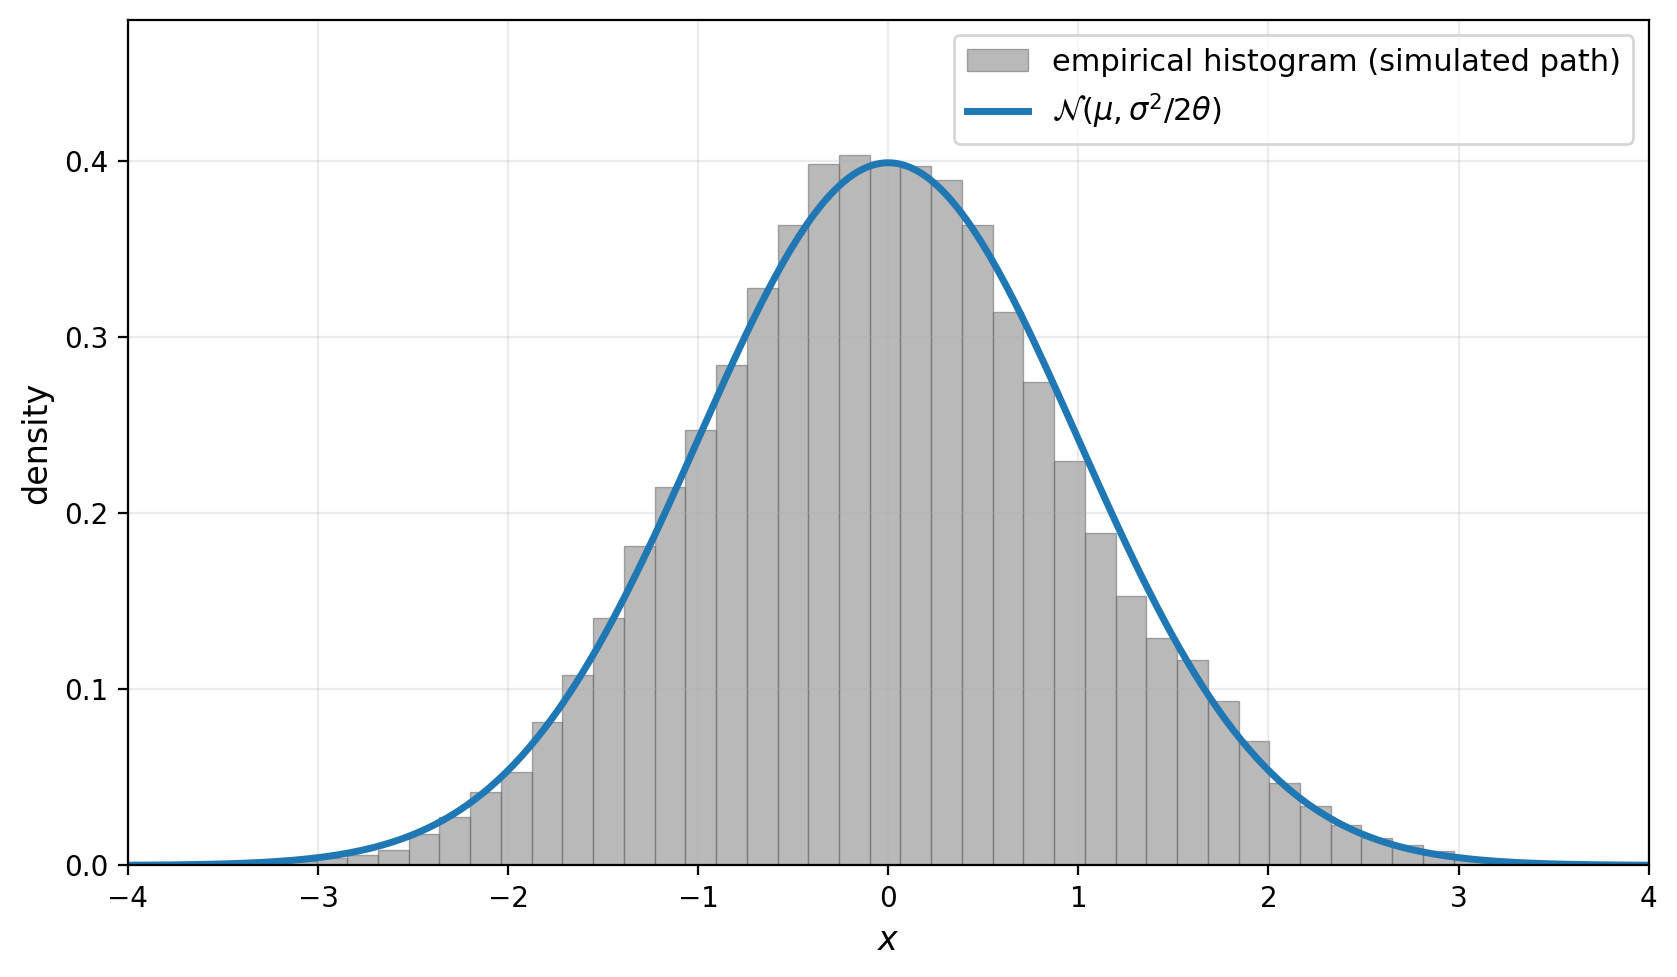
\includegraphics[width=0.85\linewidth]{figures/fig3_ou_stationary.png}
\caption{OU 过程（$\mu=0$，$\theta=0.5$，$\sigma=1$）的长程分布。直方图来自单条长模拟轨道；蓝色曲线是解析平稳密度 $\mathcal{N}(\mu,\sigma^2/2\theta)$。遍历性保证一条路径上的时间平均等于关于 $\pi$ 的空间平均。}
\label{fig:ou-stationary}
\end{figure}

\section{Feynman--Kac 公式}

向后方程可以推广到带折现和源项的情形，得到 \textbf{Feynman--Kac 公式}——它为线性抛物 PDE 的解提供随机表示。

\begin{theorem}[Feynman--Kac]\label{thm:feynmankac}
设 $a,b,r,g,f$ 光滑且有合适的有界性，$u\in C^{1,2}([0,T]\times\mathbb{R})$ 解
\[
  \begin{cases}
    \partial_t u(t,x)+\mathcal{L}u(t,x)-r(x)\,u(t,x)+g(x)=0,&(t,x)\in[0,T)\times\mathbb{R},\\
    u(T,x)=f(x).
  \end{cases}
\]
则
\[
  u(t,x)=\mathbb{E}_{t,x}\!\left[f(X_T)\,e^{-\int_t^T r(X_s)\,\mathrm{d}s}+\int_t^T g(X_s)\,e^{-\int_t^s r(X_\tau)\,\mathrm{d}\tau}\,\mathrm{d}s\right],
\]
其中 $X$ 解 \eqref{eq:sde}。
\end{theorem}

\begin{proof}
考虑过程
\[
  M_s=u(s,X_s)\,e^{-\int_t^s r(X_\tau)\,\mathrm{d}\tau}+\int_t^s g(X_\tau)\,e^{-\int_t^\tau r(X_u)\,\mathrm{d}u}\,\mathrm{d}\tau,\qquad s\in[t,T].
\]
对 $u(s,X_s)\,e^{-\int_t^s r\,\mathrm{d}\tau}$ 用 It\^o 公式，再加上第二项的微分，漂移部分压缩成 $(\partial_t u+\mathcal{L}u-ru+g)(s,X_s)\,e^{-\int}=0$（由 PDE）。故 $M$ 是（局部）鞅。

在有界性假设下 $M$ 是真鞅，所以 $\mathbb{E}_{t,x}M_t=\mathbb{E}_{t,x}M_T$。左边是 $u(t,x)$，右边正是定理中的括号项（注意 $u(T,X_T)=f(X_T)$）。
\end{proof}

II 篇里弱收敛证明引用而未证明的引理，正是 $r=g=0$ 这个特例。Feynman--Kac 在两个方向上推广了它：
\begin{itemize}
    \item 乘性折现 $e^{-\int r}$ 允许“位置依赖的杀伤”或“持有成本”；
    \item 加性源 $g$ 允许持续的现金流。
\end{itemize}

\paragraph{例：几何布朗运动下的定价。}
Black--Scholes 设定取 $\mathrm{d}S_t=rS_t\,\mathrm{d}t+\sigma S_t\,\mathrm{d}B_t$（在风险中性测度下——下一节解释这是什么意思）。在 $T$ 时刻支付 $f(S_T)$ 的欧式期权，其 $t$ 时刻价格为
\[
  V(t,S)=e^{-r(T-t)}\,\mathbb{E}[f(S_T)\mid S_t=S].
\]
用 Feynman--Kac（常数 $r$，$g=0$），$V$ 满足
\[
  \partial_t V+rS\,\partial_S V+\tfrac{1}{2}\sigma^2 S^2\,\partial_{SS}^2 V-rV=0,
\]
也就是 \textbf{Black--Scholes 方程}。封闭形式的 Black--Scholes 公式只是把 $f(S)=(S-K)^+$ 代入条件期望、利用 $S_T$ 的对数正态性算出来的。

\section{Girsanov 定理：通过对概率重新加权来改变漂移}

最后讲一个在金融和统计里不可或缺、但\emph{没有} PDE 对应物的结果：在合适的测度变换下，SDE 的漂移可以被任意修改，而它（在新测度下）仍然由一个布朗运动驱动。

\subsection{Doleans--Dade 指数}

给定适应过程 $\theta$，$\mathbb{E}\!\int_0^T \theta_s^2\,\mathrm{d}s<\infty$，定义
\[
  Z_t=\exp\!\left(\int_0^t\theta_s\,\mathrm{d}B_s-\tfrac{1}{2}\!\int_0^t\theta_s^2\,\mathrm{d}s\right).
\]
It\^o 公式给出 $\mathrm{d}Z_t=Z_t\,\theta_t\,\mathrm{d}B_t$，所以 $Z$ 是正的局部鞅，$Z_0=1$。但它不一定是\emph{真}鞅，这需要例如 \textbf{Novikov 条件}：
\[
  \mathbb{E}\exp\!\left(\tfrac{1}{2}\!\int_0^T\theta_s^2\,\mathrm{d}s\right)<\infty.
\]
满足 Novikov 条件时 $\mathbb{E}Z_T=1$，于是 $Z_T$ 可以当 Radon--Nikodym 密度用。

\subsection{Girsanov 定理}

\begin{theorem}[Girsanov]\label{thm:girsanov}
设 Novikov 条件成立。在 $(\Omega,\mathcal{F}_T)$ 上定义新概率测度 $\mathbb{Q}$：
\[
  \frac{\mathrm{d}\mathbb{Q}}{\mathrm{d}\mathbb{P}}\bigg|_{\mathcal{F}_T}=Z_T.
\]
则过程
\[
  \widetilde{B}_t=B_t-\int_0^t\theta_s\,\mathrm{d}s
\]
在 $\mathbb{Q}$ 下、$[0,T]$ 上是标准布朗运动。
\end{theorem}

\begin{proof}[证明（思路）]
$\widetilde{B}$ 在 $\mathbb{Q}$ 下是布朗运动等价于：连续（显然）、二次变差为 $t$（显然，有界变差的漂移不贡献）、是 $\mathbb{Q}$-鞅（关键）。最后一条是 Bayes 型计算：对 $s<t$ 和 $A\in\mathcal{F}_s$，
\[
  \mathbb{E}_\mathbb{Q}[\widetilde{B}_t\mathbf{1}_A]=\mathbb{E}_\mathbb{P}[Z_T\widetilde{B}_t\mathbf{1}_A]=\mathbb{E}_\mathbb{P}[Z_t\widetilde{B}_t\mathbf{1}_A]
\]
（用塔性质以及 $Z$ 是 $\mathbb{P}$-鞅）。用 It\^o 公式验证 $Z_t\widetilde{B}_t$ 本身是 $\mathbb{P}$-鞅——关键是二次协变差恒等式 $\mathrm{d}[Z,\widetilde{B}]_t=Z_t\theta_t\,\mathrm{d}t$ 恰好抵消 $\widetilde{B}$ 的漂移。所以右边等于 $\mathbb{E}_\mathbb{P}[Z_s\widetilde{B}_s\mathbf{1}_A]=\mathbb{E}_\mathbb{Q}[\widetilde{B}_s\mathbf{1}_A]$。
\end{proof}

\begin{figure}[htbp]
\centering
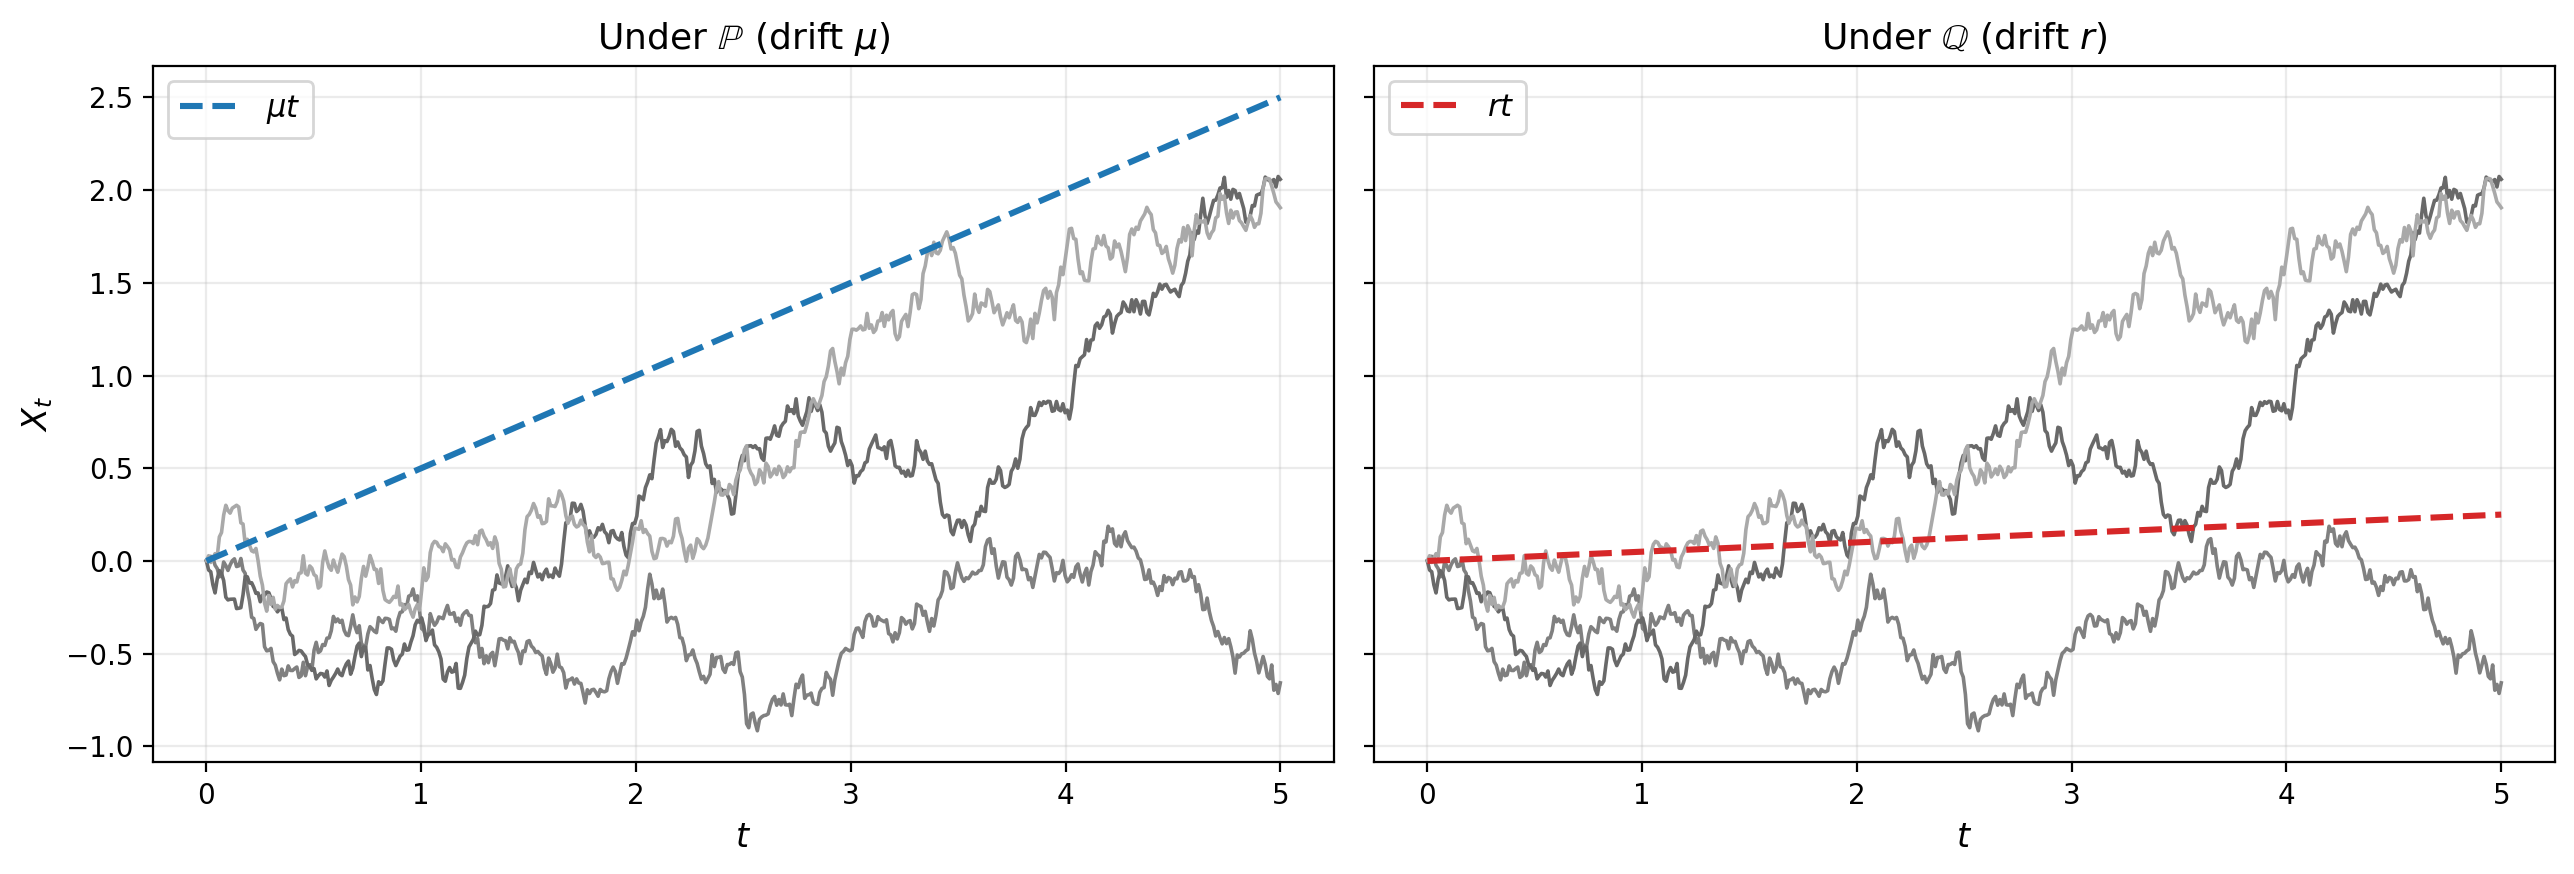
\includegraphics[width=0.95\linewidth]{figures/fig4_girsanov.png}
\caption{Girsanov 的图像。两个面板显示的是\emph{相同}的三条样本路径，区别只在概率权重：在 $\mathbb{P}$ 下它们看似“典型”（围绕趋势线 $\mu t$）；在 $\mathbb{Q}$ 下同样的路径看起来像非典型的向上偏离（趋势线变成更平缓的 $rt$）。逐路径的扩散完全一致，只有“期望趋势”的位置变了。故扩散系数 $b$ 是测度论意义上的不变量，漂移则不是。}
\label{fig:girsanov}
\end{figure}

这个解读相当震撼。在 $\mathbb{P}$ 下，SDE
\[
  \mathrm{d}X_t=a(X_t)\,\mathrm{d}t+b(X_t)\,\mathrm{d}B_t
\]
的漂移是 $a(X_t)$。选取 $\theta_t$ 满足 $b(X_t)\theta_t=\tilde a(X_t)-a(X_t)$（目标漂移为 $\tilde a$）。则在 $\mathbb{Q}$ 下：
\[
  \mathrm{d}X_t=a(X_t)\,\mathrm{d}t+b(X_t)(\mathrm{d}\widetilde{B}_t+\theta_t\,\mathrm{d}t)=\tilde a(X_t)\,\mathrm{d}t+b(X_t)\,\mathrm{d}\widetilde{B}_t.
\]
扩散系数在测度变换下不变，只有漂移在动。这是个很强的命题：它说扩散系数（更准确地说，二次变差 $[X]_t=\int_0^t b^2(X_s)\,\mathrm{d}s$）是测度论意义上的不变量，而漂移可以通过重新加权路径来调节。

\subsection{应用：风险中性定价}

Black--Scholes 模型在现实世界测度 $\mathbb{P}$ 下，股价满足 $\mathrm{d}S_t=\mu S_t\,\mathrm{d}t+\sigma S_t\,\mathrm{d}B_t$。漂移 $\mu$ 反映实际的期望收益率，通常和无风险利率 $r$ 不同。\textbf{市场风险溢价} $\lambda=(\mu-r)/\sigma$ 衡量每单位波动率对应的超额收益；把 Girsanov 参数取成它的相反数：
\[
  \theta=-\lambda=\frac{r-\mu}{\sigma},
\]
得到一个测度，在此测度下 $S$ 的漂移被平移 $\sigma\theta=r-\mu$。在 $\mathbb{Q}$ 下：
\[
  \mathrm{d}S_t=rS_t\,\mathrm{d}t+\sigma S_t\,\mathrm{d}\widetilde{B}_t.
\]
这就是\textbf{风险中性}动力学，期权定价就是把折现期望放在 $\mathbb{Q}$（而不是 $\mathbb{P}$）下计算。数学内涵是：同一个随机过程——同一组路径——承载两种同等合法的概率解读；选哪个测度，取决于你在问什么金融问题。

\section{结尾：大图景}

退一步看，本文搭出的 SDE--PDE 桥梁形成如下的图：

\begin{figure}[htbp]
    \centering
    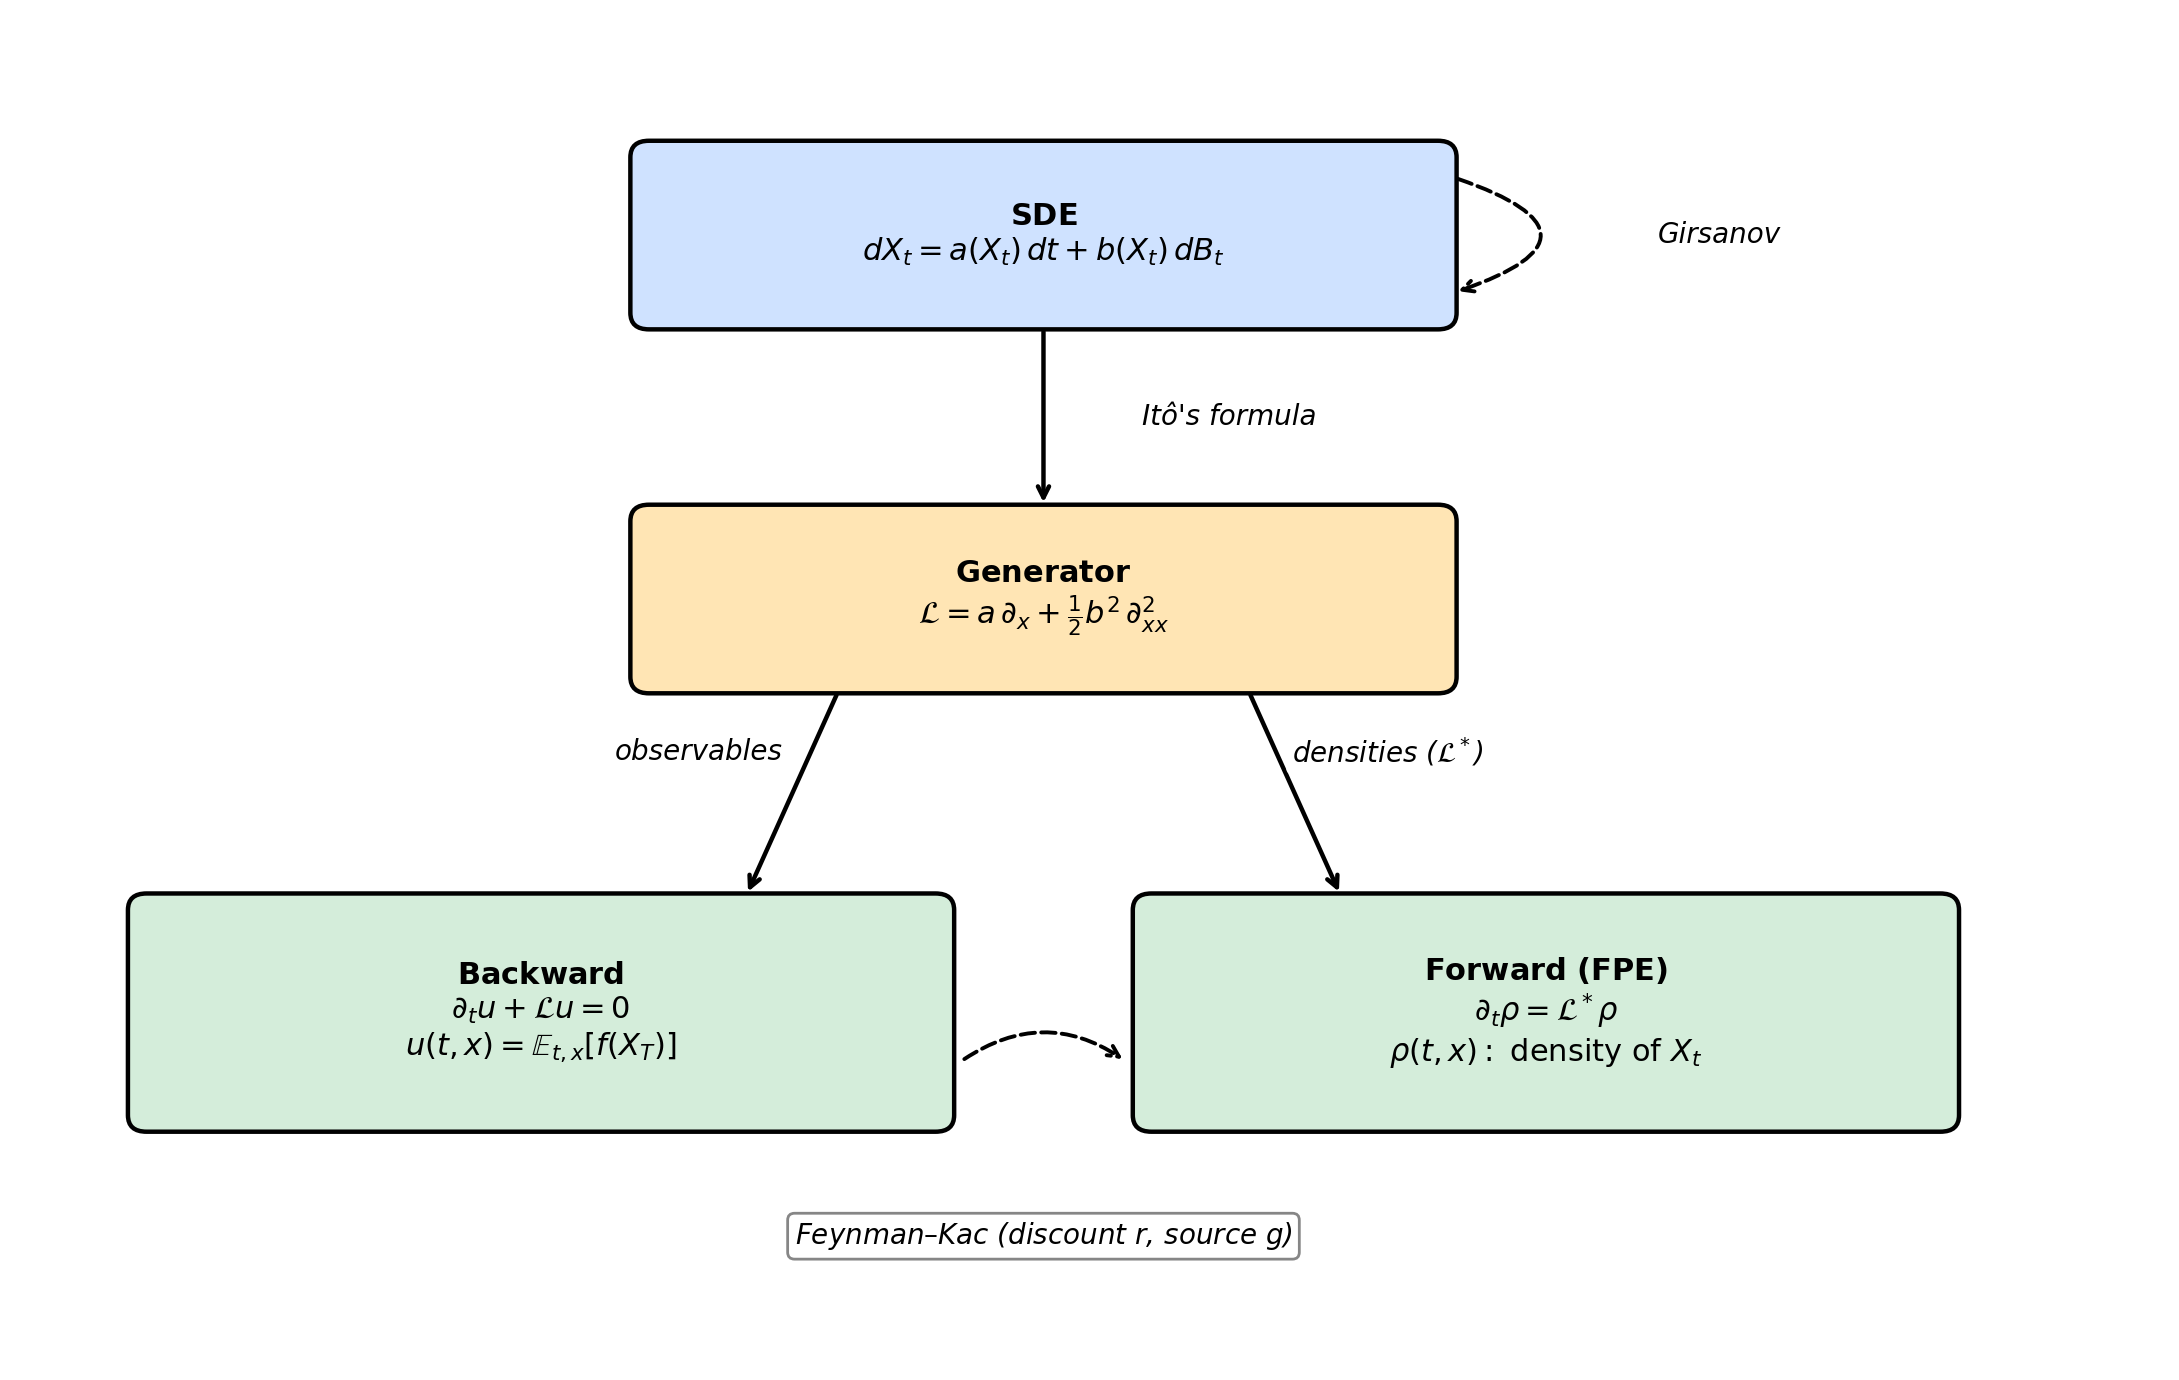
\includegraphics[width=0.9\linewidth]{figures/fig5_bridge.png}
    \caption{SDE--PDE 桥梁。由 It\^o 公式从 SDE 提取出生成元 $\mathcal L$；它产生两个对偶的 PDE：向后方程主宰可观测量的条件期望，向前方程（Fokker--Planck）主宰边际密度。Feynman--Kac 在向后方向加入折现与源项。}
    \label{fig:bridge}
\end{figure}

存在唯一性告诉我们 SDE 是良定的；马尔可夫性说解不携带超出当前状态的记忆；生成元把 SDE 提炼为一个线性算子；Kolmogorov 两个方程把这个算子翻译为关于可观测量和密度的 PDE；Feynman--Kac 给更广一类抛物方程提供随机解；Girsanov 告诉我们漂移可以调节，扩散不行。

\appendix

\section{Gronwall 不等式\label{app:gronwall}}

本文（以及 II 篇）里的证明都归结为控制一个非负函数 $\phi(t)\ge 0$，它满足如下形式的积分不等式：
\[
  \phi(t)\le \alpha+\beta\!\int_0^t\phi(s)\,\mathrm{d}s.
\]
\textbf{Gronwall 引理}（积分形式）：当 $\alpha,\beta\ge 0$ 是常数时，任何这样的 $\phi$ 满足
\[
  \phi(t)\le \alpha\,e^{\beta t}.
\]
证明只需两行：令 $\Phi(t)=\alpha+\beta\!\int_0^t\phi$，则 $\Phi'=\beta\phi\le\beta\Phi$，故 $(\Phi e^{-\beta t})'\le 0$，得 $\Phi(t)\le\Phi(0)e^{\beta t}=\alpha e^{\beta t}$；又 $\phi\le\Phi$，证毕。

SDE 应用里常需要稍一般的版本：若 $\alpha$ 是 $t$ 的非减函数，$\phi(t)\le\alpha(t)+\beta\!\int_0^t\phi(s)\,\mathrm{d}s$，则 $\phi(t)\le\alpha(t)e^{\beta t}$。证明完全相同。

\section{存在唯一性定理的细节\label{app:exuniq}}

把 Picard 迭代 Step 2 的记账补齐。定义差 $D^{(n)}_t=X^{(n+1)}_t-X^{(n)}_t$。则
\[
  D^{(n)}_t=\int_0^t\!\bigl[a(s,X^{(n)}_s)-a(s,X^{(n-1)}_s)\bigr]\mathrm{d}s+\int_0^t\!\bigl[b(s,X^{(n)}_s)-b(s,X^{(n-1)}_s)\bigr]\mathrm{d}B_s.
\]
用初等不等式 $(p+q)^2\le 2p^2+2q^2$，把 $\sup_{s\le t}$ 移到期望里面，对鞅那一项用 \textbf{Doob $L^2$ 不等式}：
\[
  \mathbb{E}\sup_{s\le t}\!\left|\int_0^s\![b(r,X^{(n)}_r)-b(r,X^{(n-1)}_r)]\mathrm{d}B_r\right|^2\le 4\mathbb{E}\!\int_0^t\!|b(r,X^{(n)}_r)-b(r,X^{(n-1)}_r)|^2\mathrm{d}r.
\]
对漂移项用 Cauchy--Schwarz，得到类似的、带 $t$ 因子的界。代入 Lipschitz 条件 (L)：
\[
  \mathbb{E}\sup_{s\le t}|D^{(n)}_s|^2\le K_1\!\int_0^t\mathbb{E}\sup_{r\le s}|D^{(n-1)}_r|^2\,\mathrm{d}s,
\]
其中 $K_1=2L^2(t+4)$ 在 $[0,T]$ 上可统一界为 $K_1=2L^2(T+4)$。迭代 $n$ 次：
\[
  \mathbb{E}\sup_{s\le T}|D^{(n)}_s|^2\le \frac{(K_1 T)^n}{n!}\,\mathbb{E}\sup_{s\le T}|D^{(0)}_s|^2,
\]
分母的阶乘最终压倒分子的指数，得到可和性。

Step 3（唯一性）是同样的计算，只是 $D=X-Y$ 为两个备选解之差：得 $\mathbb{E}\sup_{s\le t}|D_s|^2\le K_1\!\int_0^t\mathbb{E}\sup_{r\le s}|D_r|^2\,\mathrm{d}s$，Gronwall（$\alpha=0$）闭环。

\section{算子及其伴随速查\label{app:adjoint}}

对作用在光滑函数上的算子 $\mathcal{L}=a(x)\partial_x+\tfrac{1}{2}b^2(x)\partial_{xx}^2$，分部积分两次给出形式伴随
\[
  \mathcal{L}^*\rho=-\partial_x(a\rho)+\tfrac{1}{2}\partial_{xx}^2(b^2\rho),
\]
满足 $\int(\mathcal{L}u)\rho\,\mathrm{d}x=\int u(\mathcal{L}^*\rho)\,\mathrm{d}x$（边界项消失时）。$a$ 留在一次导数里、$b^2$ 处于两次导数之下，这个不对称性反映了漂移和扩散贡献的不同奇偶性，本质上跟生成元里“$a\partial_x$（一阶）$+\tfrac{1}{2}b^2\partial_{xx}^2$（二阶）”是同一件事的不同视角。

多元形式（$X_t\in\mathbb{R}^d$，$a:\mathbb{R}^d\to\mathbb{R}^d$，$b:\mathbb{R}^d\to\mathbb{R}^{d\times m}$，$\sigma=bb^\top$）：
\[
  \mathcal{L}=\sum_i a_i\,\partial_i+\tfrac{1}{2}\sum_{i,j}\sigma_{ij}\,\partial_{ij}^2,\qquad
  \mathcal{L}^*\rho=-\sum_i\partial_i(a_i\rho)+\tfrac{1}{2}\sum_{i,j}\partial_{ij}^2(\sigma_{ij}\rho).
\]
本文所有定理推广到多元情形完全一致；证明只是记号更繁，思路相同。

\clearpage % 在 CJK* 环境内输出最后一页（页眉含中文标题）
\end{CJK*}
\end{document}
